\documentclass[11pt,aspectratio=169]{beamer}
\usepackage{amsmath,amssymb,bm,booktabs,graphicx}
\usetheme{default}
\setbeamertemplate{navigation symbols}{}
\setbeamertemplate{headline}{}
\setbeamertemplate{footline}{%
  \leavevmode\hbox{%
    \begin{beamercolorbox}[wd=\paperwidth,ht=2.6ex,dp=1.1ex,right]{page number in head/foot}%
      \insertframenumber/\inserttotalframenumber\hspace{0.35cm}
    \end{beamercolorbox}}}
\setbeamertemplate{frametitle}{\vspace{0.25cm}\insertframetitle\par\vspace{0.08cm}\hrule}
\setbeamercolor{normal text}{fg=black,bg=white}
\setbeamercolor{frametitle}{fg=black,bg=white}
\setbeamercolor{structure}{fg=black}
\setbeamersize{text margin left=0.7cm,text margin right=0.7cm}
\graphicspath{{figures/}}
\newcommand{\bu}{\bm u}
\newcommand{\bv}{\bm v}
\newcommand{\bw}{\bm w}
\newcommand{\bF}{\bm F}
\newcommand{\bP}{\bm P}
\newcommand{\bI}{\bm I}
\newcommand{\bb}{\bm b}
\newcommand{\bt}{\bm t}
\newcommand{\bU}{\bm U}
\newcommand{\bR}{\bm R}
\newcommand{\bK}{\bm K}
\newcommand{\Grad}{\operatorname{Grad}}
\newcommand{\Div}{\operatorname{Div}}
\newcommand{\Vzero}{\mathcal V_0}
\newcommand{\Vhzero}{\mathcal V_{h,0}}
\DeclareMathOperator{\tr}{tr}

\begin{document}

\begin{frame}
\centering\vfill
{\LARGE\bfseries Nonlinear Finite Element Methods\par}
\vspace{0.45cm}
{\Large Lecture 3: Nonlinear Solution and Implementation\par}
\vspace{0.45cm}
Prashant K. Jha\par
ME/BME 736\par
November 10, 2026
\vfill
\end{frame}

\begin{frame}{Lecture outline}
\begin{enumerate}
\item Discretize the linearized variational equation from Lecture 2.
\item Impose correction boundary data and check convergence.
\item Introduce load stepping and step reduction.
\item Implement and check a three-dimensional hyperelastic cantilever.
\end{enumerate}
\vspace{0.3cm}
In the notebook, supply the variational forms and clamp to DOLFINx and
solve at successive loads.
\end{frame}

\begin{frame}{Recall: the linearization from Lecture 2}
We ended with the correction equation for $R=\ell_{\rm hyp}-a_{\rm hyp}$:
\[
\boxed{\delta_uR(\bu^k;\bv)[\Delta\bu^k]=-R(\bu^k;\bv)
\quad\forall\bv\in\Vzero.}
\]
Here $\bv\in\Vzero$ is held fixed, and $\delta_uR[\Delta\bu^k]$ varies
the displacement in the correction direction. The update is
\[
\bu^{k+1}=\bu^k+\Delta\bu^k.
\]
The variational equation is already linearized. We now choose FE correction
and test functions to obtain its matrix system.
\end{frame}

\begin{frame}
\centering\vfill
{\LARGE Finite element equations and Newton iteration\par}
\vspace{0.4cm}
Choose FE directions in the linearized variational equation.
\vfill
\end{frame}

\begin{frame}{Finite element displacement, correction, and test functions}
For scalar nodal basis functions $\phi_i$, write the current displacement as
\[
\bu_h^k=\sum_{i=1}^{N_n}\phi_i\bm U_i^k,\qquad
\bm U_i^k=\begin{bmatrix}U_{i1}^k&U_{i2}^k&U_{i3}^k\end{bmatrix}^{T}.
\]
Here $i,j$ label nodes and $\alpha,\beta\in\{1,2,3\}$ label displacement
components. Stack the nodal vectors into $\bU^k$.
Expand the correction and choose one test direction:
\[
\Delta\bu_h^k=\sum_{j=1}^{N_n}\sum_{\beta=1}^3
\Delta U_{j\beta}^k\phi_j\bm e_\beta,
\qquad \bv_h=\phi_i\bm e_\alpha.
\]
Use free test directions, for which $\phi_i\bm e_\alpha\in\Vhzero$.
Prescribed correction coefficients are zero.
\end{frame}

\begin{frame}{The linearized variational equation gives the matrix system}
Insert the FE correction and test direction into the recalled equation.
The derivative is linear in the correction direction, so each free row gives
\[
\sum_{j,\beta}
\underbrace{\delta_uR(\bu_h^k;\phi_i\bm e_\alpha)
[\phi_j\bm e_\beta]}_{(K_T)_{i\alpha,j\beta}}
\Delta U_{j\beta}^k
=-\underbrace{R(\bu_h^k;\phi_i\bm e_\alpha)}_{R_{i\alpha}}.
\]
These evaluations define the tangent matrix and residual vector at $\bu_h^k$:
\[
\boxed{\sum_{j,\beta}(K_T)_{i\alpha,j\beta}\Delta U_{j\beta}^k
=-R_{i\alpha}\quad\text{on free rows}.}
\]
This is the FEniCSx sequence: differentiate the residual form, then assemble.
The test function supplies the row direction; the trial correction supplies
the column direction. Next, impose the prescribed correction coefficients.
\end{frame}

\begin{frame}{Free equations, prescribed corrections, and reactions}
Partition coefficients into free ($f$) and prescribed ($p$) entries.
Initialize $\bU_p^k=\overline{\bU}_p$.
Keeping these prescribed values fixed requires
$\Delta\bU_p^k=\overline{\bU}_p-\bU_p^k=\bm0$.
The free Newton rows are
\[
(K_T)_{ff}\Delta\bU_f^k
+(K_T)_{fp}\underbrace{\Delta\bU_p^k}_{\bm0}
=-\bR_f(\bU^k).
\]
Therefore solve and update
\[
\boxed{(K_T)_{ff}\Delta\bU_f^k=-\bR_f(\bU^k),\qquad
\bU_f^{k+1}=\bU_f^k+\Delta\bU_f^k.}
\]
Keep $\bU_p^{k+1}=\overline{\bU}_p$. Evaluate the residual using the full
current vector, including prescribed coefficients.

After convergence, the support reactions are $\bm r_p=-\bR_p$ from the
unmodified residual. Prescribed residual entries are not required to vanish.
\end{frame}

\begin{frame}{Newton algorithm at a fixed load}
\begin{enumerate}
\item Initialize the full coefficient vector with the prescribed values and
an admissible deformation.
\item Assemble $\bR(\bU^k)$ and check its free entries for convergence.
\item If not converged, assemble $\bK_T(\bU^k)$ and solve
\[
(K_T)_{ff}\Delta\bU_f^k=-\bR_f(\bU^k).
\]
\item Form a trial update, retaining the prescribed coefficients. Accept a
suitable step, then reevaluate the nonlinear residual.
\item Repeat until convergence or the iteration limit. Report failure if the
solve does not converge.
\end{enumerate}
Each iteration uses the stress and tangent at the current displacement.
We next specify a stopping test and how to reduce an unsuitable update.
\end{frame}

\begin{frame}{Stopping the nonlinear iteration}
Check only the free equations. One absolute-and-relative force criterion is
\[
\boxed{\|\bR_f(\bU^k)\|_2
\leq\varepsilon_{\rm abs}
+\varepsilon_{\rm rel}\|\bR_f(\bU^0)\|_2.}
\]
Here $\bU^0$ is the initial iterate at this load,
$\varepsilon_{\rm abs}$ has force units, and $\varepsilon_{\rm rel}$ is
dimensionless.
\begin{itemize}
\item A small correction alone is insufficient. Evaluate the residual after
updating to check the actual force imbalance.
\item Convergence solves the equations on the chosen mesh. Mesh accuracy
requires a separate refinement study.
\end{itemize}
For a smooth residual, a nonsingular free Jacobian, and a sufficiently close
initial guess, full Newton steps give local quadratic convergence.
\end{frame}

\begin{frame}{Load stepping}
Introduce a load factor $\zeta\in[0,1]$:
\[
R_\zeta(\bu;\bv)
=\zeta\ell_{\rm hyp}(\bv)-a_{\rm hyp}(\bu;\bv).
\]
For example, solve at $\zeta=0.25,\ 0.50,\ 0.75,\ 1.00$.
\begin{enumerate}
\item Set the target load factor.
\item Start Newton iteration from the previous converged displacement.
\item Converge at this load before advancing to the next one.
\end{enumerate}
The load factor changes between solves. It stays fixed during each Newton
iteration. If a load step fails, reduce its increment and retry from the last
converged state.

This is a sequence of quasistatic equilibria, not time integration.
\end{frame}

\begin{frame}{Step reduction within a Newton solve}
After computing $\Delta\bU^k$, test
\[
\bU_{\rm trial}=\bU^k+\omega\Delta\bU^k,
\qquad 0<\omega\leq1.
\]
The step must stay in the domain of the material law. For this model,
$J=\det\bF$ must be positive to evaluate $\ln J$.
Backtracking reduces $\omega$ when the residual does not decrease enough.
\[
\|\bR_f(\bU_{\rm trial})\|_2<\|\bR_f(\bU^k)\|_2
\qquad\text{is a simple decrease test.}
\]
In the demo, PETSc performs the line search. We check $J$ at the
converged state, rather than assuming the line search guarantees $J>0$
at all trial states.
\end{frame}

\begin{frame}
\centering\vfill
{\LARGE FEniCSx implementation\par}
\vspace{0.4cm}
A hyperelastic cantilever solved at successive loads.
\vfill
\end{frame}

\begin{frame}{Example: a three-dimensional hyperelastic cantilever}
\[
\Omega_0=(0,4)\times(0,1)\times(0,1)\ \mathrm{mm}^3,
\qquad \mu=1\ \mathrm{MPa},\quad\lambda=2\ \mathrm{MPa}.
\]
\begin{columns}[c,onlytextwidth]
\begin{column}{.56\textwidth}
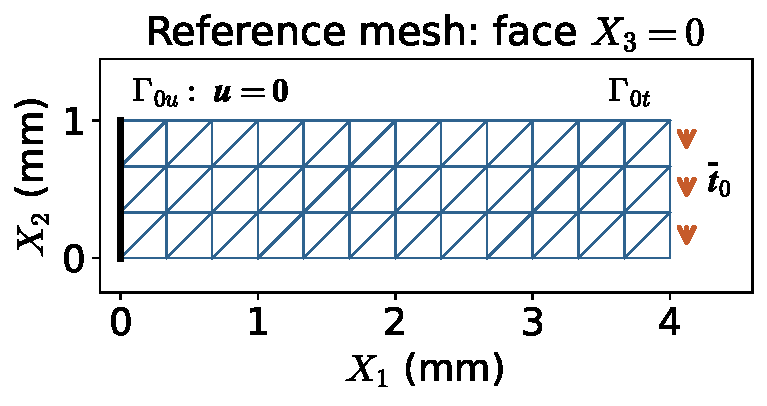
\includegraphics[width=\textwidth]{beam_setup.pdf}
\end{column}
\begin{column}{.41\textwidth}
No body force. The strong problem is
\[
\begin{aligned}
-\Div\bP&=\bm0&&\text{in }\Omega_0,\\
\bu&=\bm0&&\text{on }\Gamma_{0u},\\
\bP\bm N&=\zeta\bt_*&&\text{on }\Gamma_{0t},
\end{aligned}
\]
where $\bt_*=(0,-0.02,0)^T$ MPa.
The other four faces have zero traction.
\end{column}
\end{columns}
$\Gamma_{0u}$ is $X_1=0$, $\Gamma_{0t}$ is $X_1=4$ mm, and $\bm N$ is the
reference outward normal. The solve uses 3D tetrahedra.
\end{frame}

\begin{frame}[fragile]{Energy and automatic differentiation}
Use $\bF=\bI+\Grad\bu$, $J=\det\bF$, and
\[
\Psi=\frac\mu2\bigl(\tr(\bF^T\bF)-3\bigr)
-\mu\ln J+\frac\lambda2(\ln J)^2.
\]
For this body, with no body force,
\[
\Pi_\zeta(\bu)=\int_{\Omega_0}\Psi\,\mathrm dV_0
-\zeta\int_{\Gamma_{0t}}\bt_*\cdot\bu\,\mathrm dA.
\]
In the notebook, \texttt{u} is the current FE displacement, \texttt{v} the
test function, and \texttt{w} the trial correction direction:
\begin{verbatim}
Pi = psi*dx - load*ufl.dot(traction, u)*ds(1)
residual = -ufl.derivative(Pi, u, v)
tangent = ufl.derivative(residual, u, w)
\end{verbatim}
These lines implement $R=-\delta\Pi$ and its derivative $\delta_uR$.
\end{frame}

\begin{frame}[fragile]{The nonlinear solve in DOLFINx}
Use \texttt{fem.dirichletbc} to prescribe zero displacement at the clamp.
Pass that condition and the two UFL forms to \texttt{NonlinearProblem}.
\begin{verbatim}
problem = NonlinearProblem(
    residual, u, J=tangent, bcs=[bc],
    petsc_options_prefix="cantilever_",
    petsc_options=solver_options,
)

for zeta in load_factors:
    load.value = zeta
    problem.solve()
\end{verbatim}
The notebook selects Newton with backtracking and a direct linear solve.
DOLFINx assembles the forms and applies the clamp; PETSc solves the nonlinear
equations. The solution in \texttt{u} starts the next load step.
\end{frame}

\begin{frame}{Computed load response}
The loaded reference area is $A_0=1\ \mathrm{mm}^2$.
Define the mean downward displacement of the loaded face by
\[
d_{\rm end}=-\frac1{A_0}\int_{\Gamma_{0t}}u_2\,\mathrm dA.
\]
\begin{center}
\begin{tabular}{rrr}
\toprule
$\zeta$ & Newton iterations & $d_{\rm end}$ (mm)\\
\midrule
0.25 & 20 & 0.330589\\
0.50 & 20 & 0.651313\\
0.75 & 20 & 0.952931\\
1.00 & 20 & 1.229509\\
\bottomrule
\end{tabular}
\end{center}
At full load the minimum element determinant is $0.922265$.
The solve converged on this mesh; a refinement study would test mesh accuracy.
\end{frame}

\begin{frame}{Load response and Newton convergence}
\begin{center}
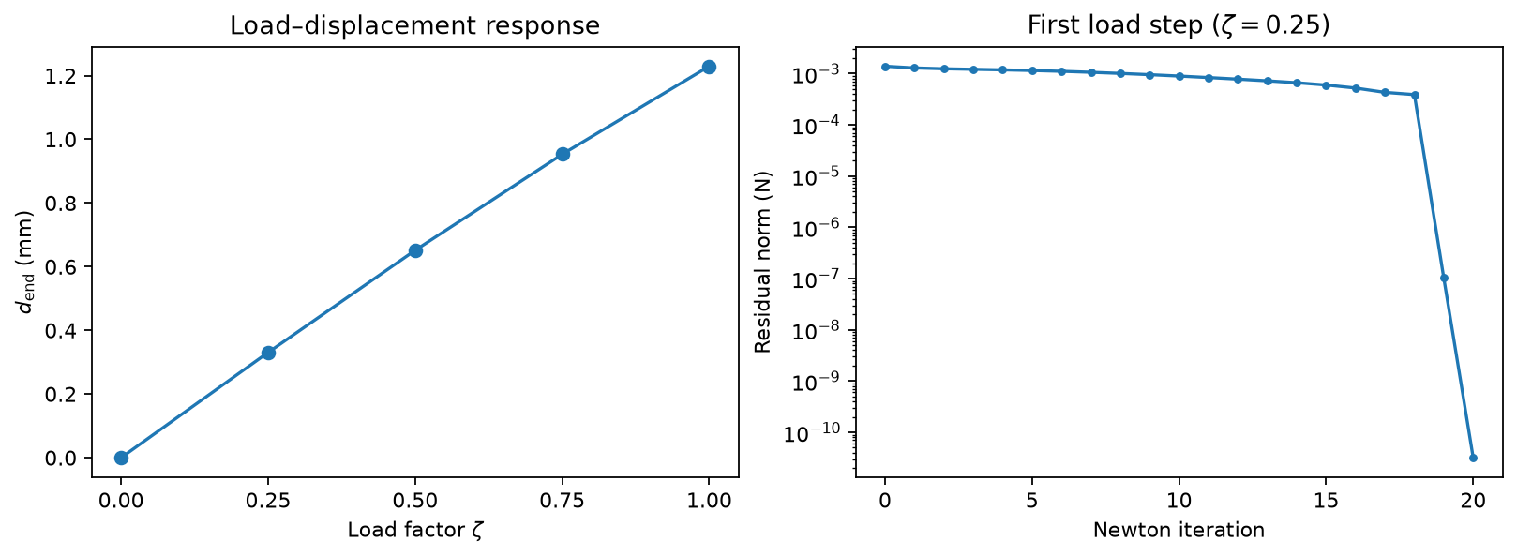
\includegraphics[width=\textwidth]{beam_response.pdf}
\end{center}
Each point on the left is a converged load step, with the unloaded state at
the origin. On the right, PETSc records the residual norm during the first
load step, with the load held fixed.
\end{frame}

\begin{frame}{Deformed cantilever at two loads}
\begin{center}
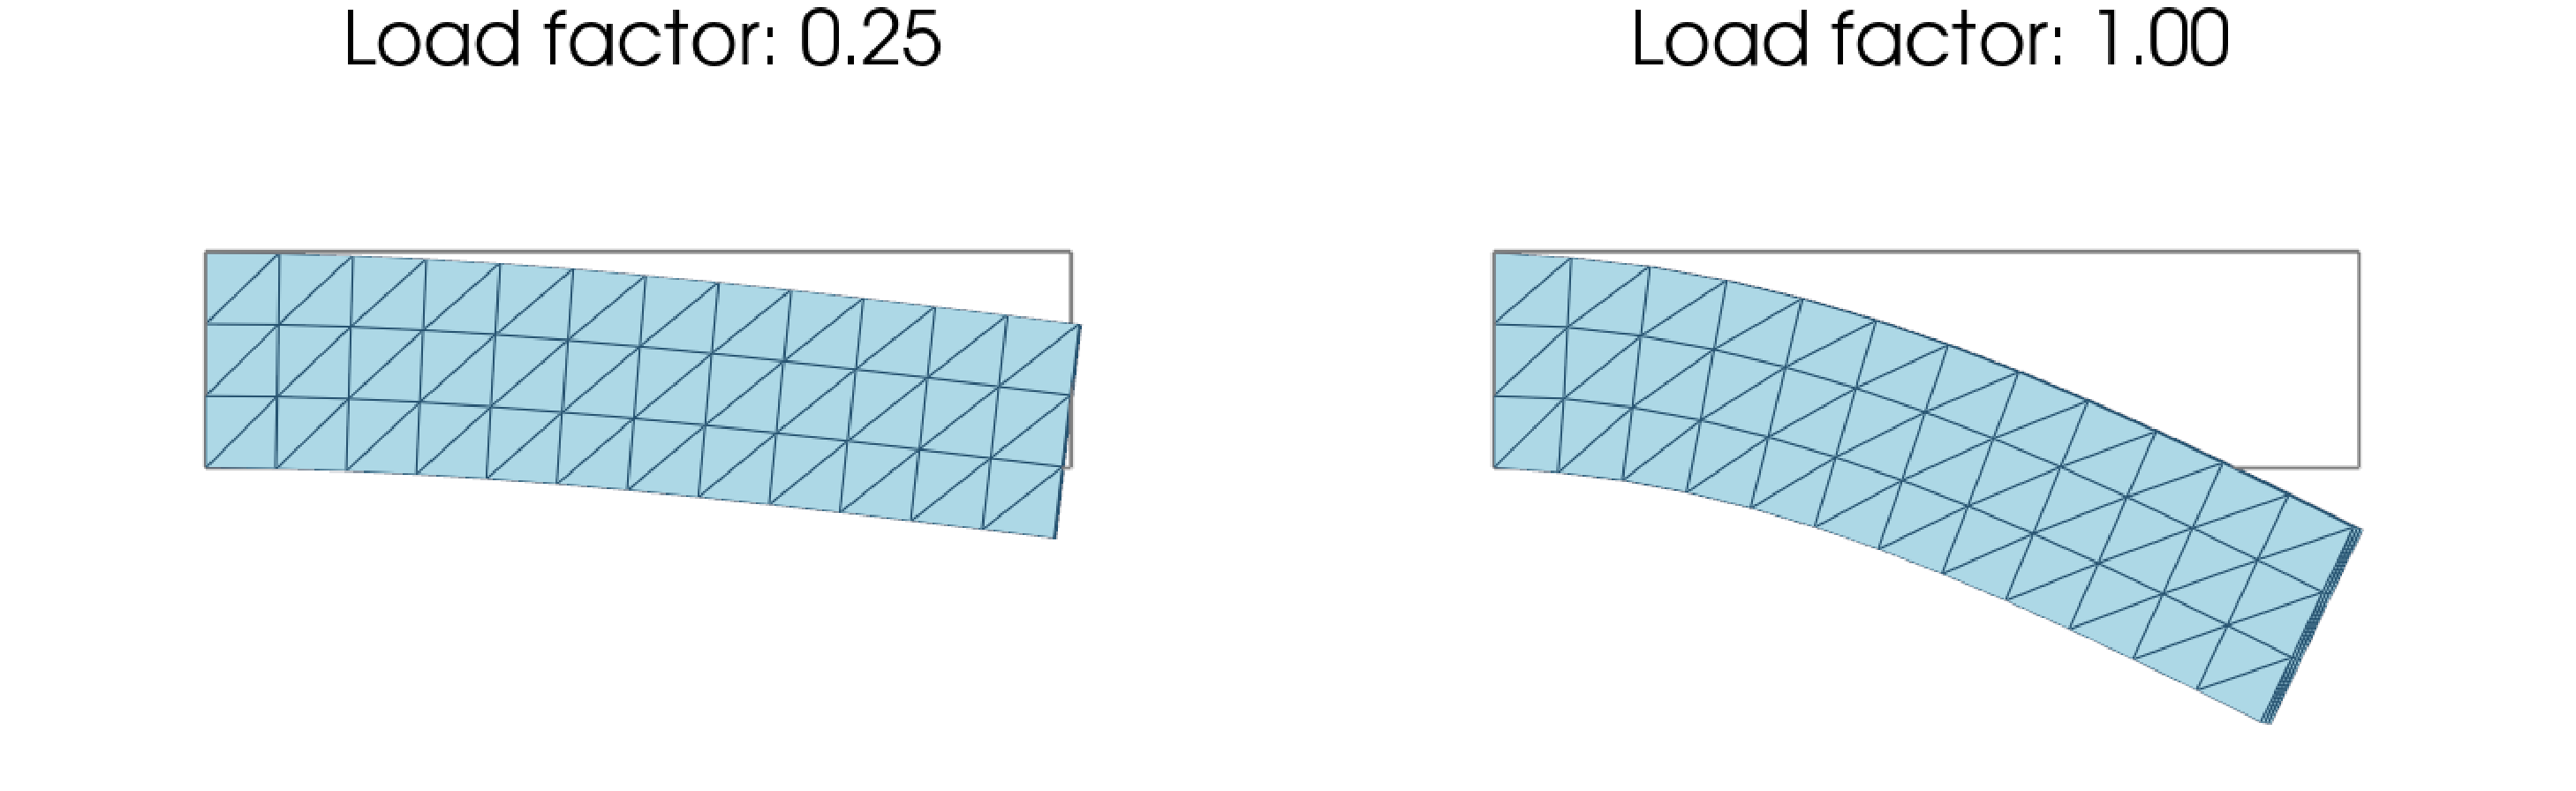
\includegraphics[width=\textwidth]{beam_deformation.pdf}
\end{center}
The gray outline is the reference beam. The blue mesh shows
$\bm x=\bm X+\bu$ at each load, with no displacement magnification.
Both panels use the same side view and scale.
\end{frame}

\begin{frame}{Summary and reading}
\begin{itemize}
\item Use $R=\ell-a$ in the variational and assembled equations.
\item Linearize the variational residual, assemble its tangent, and solve
$(K_T)_{ff}\Delta\bU_f=-\bR_f$, with zero prescribed correction.
\item Reassemble at each new displacement. Use load stepping and reduce an
unsuitable Newton step.
\item UFL supplies $R=-\delta\Pi$ and its tangent. Pass those forms and the
boundary condition to DOLFINx's nonlinear solver.
\end{itemize}
\vspace{0.15cm}
\href{../../../notebooks/nonlinear/hyperelasticity_newton.ipynb}{Companion notebook: hyperelasticity\_newton.ipynb.}

\small
Course book, Chapter 9, \S\S9.3--9.8.
Belytschko--Moran \emph{Solution Methods} notes, \S\S6.3.3--6.3.8,
printed pp.~6-9--6-22.
\href{https://docs.fenicsproject.org/dolfinx/main/cpp/demos/demo_hyperelasticity.html}{DOLFINx hyperelasticity example}
and \href{https://docs.fenicsproject.org/dolfinx/v0.11.0/python/generated/dolfinx.fem.petsc.html\#dolfinx.fem.petsc.NonlinearProblem}{DOLFINx nonlinear solver}.
\end{frame}

\end{document}
